\documentclass[12pt]{article} 

% Adjust margining to narrow
\usepackage{geometry}
\geometry{a4paper, total={170mm,257mm}, left=20mm, top=20mm}

% Mathematics font
\usepackage{amsfonts}
\usepackage{amsmath}

% Graphics import
\usepackage{graphicx}
\usepackage{subcaption}
\graphicspath{{C:/Users/user/Desktop/KUL - Mstat/Big Data Platforms and Technologies/report/graph}}

% Advanced table
\usepackage{tabularx}
\usepackage{makecell}

% No indentation
\setlength\parindent{0pt}

% ------------------------------------------------------------------------
% Assignment content
\begin{document}
\begin{titlepage}
	\begin{center}
	\vspace*{1cm}
    
\includegraphics[width=0.4\textwidth]{KUL}
	\vspace{2.5cm}
    {\Large Report for Advanced Analytics in Business}
            
    \vspace{1.5cm}

    {\large Cheung Wai Chun, r0817438}\\
    \vspace{0.5cm}
    {\large David Badajkov, r0604517}\\
    \vspace{0.5cm}
    {\large Ana Maria Giraldo Vargas, r0822450}\\
    \vspace{0.5cm}
	{\large Sonia Rocio 	Socadagui Casas, r0823960}\\
	\vspace{0.5cm}
	{\large Marcela 	Lopez Viveros, r0773141}
	\vspace{1.5cm}

       \today
   \end{center}
\end{titlepage}

% ------------------------------------------------------------------------
\newpage
\tableofcontents
\newpage

\section*{Assignment 1}
\addcontentsline{toc}{section}{Assignment 1}


\subsection*{Feature engineering}
\addcontentsline{toc}{subsection}{Feature engineering}

The dataset for Assignment 1 consists of 55463 observations and 78 features. The number of features. It is easy to observe that there are a lot of missing values and categorical or date features in the dataset. In this section, we would discuss the strategies used in handling such problems. 

\subsubsection*{Missing values}
\addcontentsline{toc}{subsubsection}{Missing values}

As shown in figure 1, there are 55 feature which contain missing values, and 24 out of them contain more than 80\% of missing values. For those features with a high proportion of missing values (more than 50\%), missing values are treated as an extra category. By treating missing values as an extra category, the information of the non-missing entries of those features can be retained and learnt by the model, whereas removal of those features may lead to a loss in information or pattern.  

\begin{figure}[h]
\centering
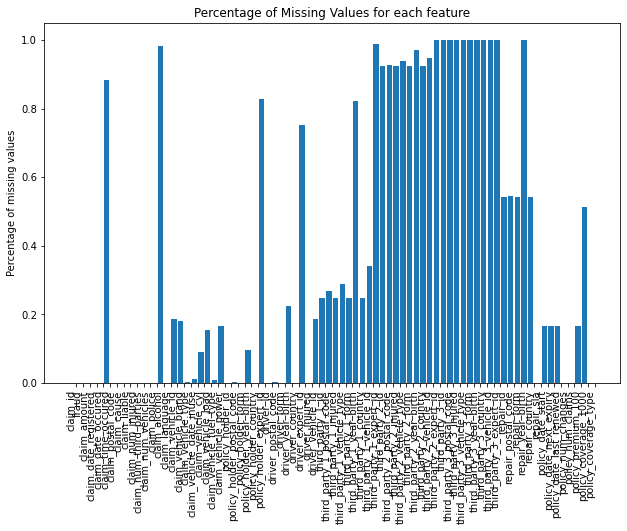
\includegraphics[width=1\linewidth]{missing_value_plt1}
\caption{Proportions of missing values for each feature}
\end{figure}

\subsection*{Exploratory data analysis}
\addcontentsline{toc}{subsection}{Exploratory data analysis}

\subsection*{Model building}
\addcontentsline{toc}{subsection}{Model building}

\subsection*{Interpretation}
\addcontentsline{toc}{subsection}{Interpretation}

\subsection*{Reflection}
\addcontentsline{toc}{subsection}{Reflection}

\section*{Assignment 2}
\addcontentsline{toc}{section}{Assignment 2}

\section*{Assignment 3}
\addcontentsline{toc}{section}{Assignment 3}

\section*{Assignment 4}
\addcontentsline{toc}{section}{Assignment 4}
\end{document}